\chapter{Theoretical Foundations}

% measurement of spin observables is challenging but rewarding
%   examples?
% 

\section{The Simple Parton Model}

% predates QCD, invented to explain scaling of F_{1,2}
% Leader cites 69 Feynman PRL as inventor of parton model, but I skimmed the Letter and I don't see it.
% \cite{Panofsky:1968pb} -- confirmation of Bjorken scaling
% \cite{Bjorken:1968dy} -- Bjorken scaling

In the late nineteen-sixties high energy physicists at SLAC confirmed Bjorken's
hypothesis that the inelastic structure functions of the proton scaled; that is,
at high energies they did not depend on the $Q^2$ of the interaction. This
result stood in sharp contrast to the power-law behavior of the proton's elastic
form factors, and implied the existence of point-like constituents inside the
proton. These ``partons'' were conceived as effectively massless,
electromagnetically charged particles; in the deep-inelastic scattering
(DIS) regime, a virtual photon interacts with a parton, not the proton as a
whole.

Scaling is manifest when Bjorken's $F_1$ structure function is expressed in terms of the number densities $q(x)$ of quarks and $\bar q(x)$ of antiquarks as
%
\begin{equation}
  F_1(x, Q^2) = \frac{1}{2}\sum_{j}{e_j^2[q_j(x) + \bar{q}_j(x)]}
\end{equation}
%
where the sum is taken over quark flavors $j$ and $e_j$ is the electromagnetic charge of flavor $j$.  In longitudinally polarized DIS we define a polarization density $\Delta  q(x) \equiv q_+(x) - q_-(x)$ as the difference in number density between quarks whose spins are aligned with the (longitudinal) spin of the proton and quarks whose spins are anti-aligned; the polarized analogue to $F_1$ is then
%
\begin{equation}
  g_1(x, Q^2) = \frac{1}{2}\sum_{j}{e_j^2[\Delta q_j(x) + \Delta \bar{q}_j(x)]}.
\end{equation}

In the naive parton model we assume $SU(3)_F$ flavor symmetry and thus it is useful to rewrite the expression for $g_1$ in terms of quantities which have specific $SU(3)_F$ transformation properties:
%
\begin{equation}
  g_1(x) = \frac{1}{9}[\frac{3}{4}\Delta q_3(x) + \frac{1}{4}\Delta q_8(x) + \Delta \Sigma(x)]
\end{equation}
%
where
%
\begin{eqnarray}
  \Delta q_3 & = & (\Delta u + \Delta \bar{u}) - (\Delta d + \Delta \bar{d}) \nonumber \\
  \Delta q_8 & = & (\Delta u + \Delta \bar{u}) + (\Delta d + \Delta \bar{d}) - 2(\Delta s + \Delta \bar{s}) \nonumber \\
  \Delta \Sigma & = & (\Delta u + \Delta \bar{u}) + (\Delta d + \Delta \bar{d}) + (\Delta s + \Delta \bar{s})
  \label{eqn:su3_dis}
\end{eqnarray}
%
The first moments of these quantities are the hadronic matrix elements of an octet of quark $SU(3)_F$ axial-vector currents $J_{5\mu}^i$ and a flavor singlet singlet axial current $J_{5\mu}^0$.  In the limit of massless partons the non-singlet currents are conserved quantities, and are known from $\beta$-decay measurements:
%
\begin{eqnarray}
  a_3 & = & \int_0^1 dx~\Delta q_3(x) = g_A = 1.2670 \pm 0.0035 \nonumber \\
  a_8 & = & \int_0^1 dx~\Delta q_8(x) = 0.585 \pm 0.025
\end{eqnarray}
%
A measurement of the first moment of $g_1^p$ could thus be interpreted as a measurement of the singlet current $a_0 = \int_0^1 dx~\Delta \Sigma (x)$, and in turn as a measurement of the quark spin contribution to the spin of the proton.  We rearrange \ref{eqn:su3_dis} to yield an expression for $a_0$ in terms of $a_8$ and the polarized strange quark densities:
%
\begin{equation}
  a_0 = a_8 + 3 \int_0^1 dx~(\Delta s + \Delta \bar s)
  \label{eqn:a_0_prediction}
\end{equation}
%
If one assumes that the sea quark distribution is either unpolarized or CP-symmetric and thus does not contribute to the spin of the proton, Equation \ref{eqn:a_0_prediction} becomes a \textit{prediction} for $\langle S_z \rangle$, as noted by Ellis and Jaffe \cite{Ellis:1973kp} in 1974.

% Should say something about the Sehgal result \cite{Sehgal:1974rz} that concludes the quark contribution to the spin of the proton is $\sim$ 0.3, in agreement with Ellis-Jaffe but using a slightly different derivation (Bjorken sum rule \cite{Bjorken:1966jh}, equivalent parton model result (cites several people), use SU(3) symmetry to obtain same result for $\Xi^- (dss) \rightarrow \Xi^0 (uss) + e + \bar \nu_e$, expresses $\frac{G_A}{G_V}$ ratios in terms of experimentally-measurable quantities $F$ and $D$ (calls that step the octet-model results), seems that $F+D = \frac{G_A}{G_V} \approx g_A = a_3$, F/D 

% In much of the literature I see $g_A$ instead of Griffiths' $\frac{G_A}{G_V}$.  I wonder if that is a definition, or if the literature just takes the Conserved Vector Current hypothesis $G_V = 1$ for granted? -- yes, it's the latter, see Stiegler 1995

% \begin{equation}
%   \Gamma_1^p \equiv \int_0^1 dx~g_1(x) = \frac{1}{9}[\frac{3}{4}a_3 + \frac{1}{4}a_8 + a_0]
% \end{equation}

% \begin{eqnarray*}
%   a_3 \equiv g_A & = & 1.2670 \pm 0.0035 \\
%   a_8 & = & 0.585 \pm 0.025
% \end{eqnarray*}

% really should mention Bjorken's sum rule in here somewhere, since its definitely true and not model dependent
% Bjorken sum rule -- what do I need to say about it?
% \begin{equation}
%   \int_0^1 dx~g_1^p(x,Q^2) - g_1^n(x,Q^2) = \frac{g_A}{6}(1 + O(\alpha_s))
% \end{equation}

\section{First Experimental Tests}

In polarized deep inelastic scattering, a longitudinally polarized lepton beam is scattered off of nucleon targets polarized parallel or perpendicular to the beam axis. Asymmetries are formed by comparing event rates for scattering in different spin configurations.  For a spin $\frac{1}{2}$ target, the asymmetries of interest are

% Stiegler does not include the 1/2 nor the differential in this equation
\begin{equation}
  A_{\parallel} = \frac{d\sigma^{\rightarrow \Leftarrow} - d\sigma^{\rightarrow \Rightarrow}}{2d\sigma_{unpol}}, ~~~~~~~
  A_{\perp} = \frac{d\sigma^{\rightarrow \Uparrow} - d\sigma^{\rightarrow \Downarrow}}{2d\sigma_{unpol}}
\end{equation}

Spin-dependent cross sections can be calculated by contracting the elastic Compton amplitude $T_{\mu \nu}$ with the photon polarization vectors; in the presence of parity conservation and time reversal, four of these are independent \cite{??}:
%
\begin{eqnarray}
  \sigma_{1/2} & = & F_1 + g_1 - \gamma^2 g_2, \nonumber \\
  \sigma_{3/2} & = & F_1 - g_1 + \gamma^2 g_2, \nonumber \\
  \sigma_L & = & -F_1 + F_2(1+\gamma^2)/(2x),  \nonumber \\
  \sigma_{TL} & = & \sqrt{2}\gamma (g_1+g_2).
\end{eqnarray}
%
Here $\gamma^2 = Q^2/v^2$.  These four cross sections are commonly rearranged into a pair of virtual photon asymmetries $A_1$ and $A_2$:
%
\begin{equation}
  A_1 = \frac{\sigma_{1/2} - \sigma_{3/2}}{\sigma_{1/2} - \sigma_{3/2}}, ~~~~ A_2 = \frac{\sigma_{TL}}{\sigma_T}
\end{equation}
%
The longitudinal and transverse DIS asymmetries can then be written in terms of these virtual photon asymmetries,
\begin{equation}
  A_{\parallel} = D(A_1 + \eta A_2), ~~~~~ A_{\perp} = d(A_2 - \xi A_1)
\end{equation}
%
where the coefficients $D$, $\eta$, $d$, and $\xi$ can be approximated to first order in $\gamma$ in terms of the usual DIS kinematic variables and $R = \frac{\sigma_{TL}}{\sigma_T}$:
\begin{eqnarray}
  D & \approx & \frac{y(2-y)}{y^2 + 2(1-y)(1+R)}, ~~~~~~~~ \eta \approx \frac{2(1-y)}{y(2-y)} \frac{\sqrt{Q^2}}{E} \nonumber \\
  d & \approx & D \frac{\sqrt{1-y}}{1-y/2}, ~~~~~~~~ \xi \approx \gamma(1-\frac{y}{2})
\end{eqnarray}
%
$D$ can be thought of as a depolarization factor arising from the fact that the photon is not fully aligned with the lepton beam, and $\eta$, $\xi$ are kinematic factors that are usually small.  The structure functions can also be written in terms of $A_{1,2}$:
\begin{equation}
  g_1 = \frac{F_2}{2x(1+R)}(A_1+\gamma A_2), ~~~~~ g_2 = \frac{F_2}{2x(1+R)}(A_2/\gamma - A_1).
\end{equation}
Thus, measurements of $A_{\parallel}$, $A_{\perp}$, $F_2$, and $R$ are sufficient to extract the polarized structure functions of the nucleon.

% \begin{equation}
%   \gamma = \sqrt{\frac{2Mx}{Ey}}
% \end{equation}

% note that they just measured A_parallel and neglected the A_2 contribution
The first DIS experiments to extract $g_1$ were E80 and E130, conducted in the early 1980s at SLAC.  These experiments scattered longitudinally polarized electron beams off of longitudinally polarized proton targets and were able to measure $A_1^p$ in the range $0.1 < x < 0.7$.  Their results were consistent with expectations from the parton model in that limited kinematic regime.

In 1988, the European Muon Collaboration (EMC) published data on asymmetries of longitudinally polarized \textit{muon} beams scattering off of longitudinally polarized proton targets.  

From these data they extracted measurements of the proton's $g_1$ structure function over a wide range in $x$ and $Q^2$.  As shown in Figure \ref{fig:emc-g1p}, the integral value of $g_1^p$ obtained from that extraction was incompatible with the prediction from Ellis and Jaffe.

% measured asymmetry


\begin{equation}
  A_1 = (g_1 - \gamma^2 g_2)\frac{1}{F_1}, ~~~~~~~~ A_2 = \gamma(g_1+g_2)\frac{1}{F_1}
\end{equation}

\begin{figure}
  \includegraphics[width=1.0\textwidth]{figures/emc-g1p}
  \caption{EMC extraction of $g^1_p$ and its integral compared to the prediction from Ellis-Jaffe \cite{Ashman:1987hv}}
  \label{fig:emc-g1p}
\end{figure}

\begin{equation}
  A_1 \approx \frac{A_{\parallel}}{D} \approx (1 + \gamma^2)\frac{g_1}{F_1}
\end{equation}

EMC measures first moment of g1, taking a3 and a8 from beta-decay measurements means that we can extract a0 from $\Gamma_1^p$ and it's $\sim$ 0.  But

\begin{equation}
  a_0 = \Delta \Sigma = a_8 + 3(\Delta s + \Delta \bar{s})
\end{equation}

from above, and if you ignore strange quark contributions (Ellis-Jaffe) you get $a_0 \sim 0.59$, obviously in stark contrast to EMC.  This is the original ``spin crisis''.  And of course $a_0 = 2<S_z^{quarks}>$.

Any need to mention ``Cloudy Bag'' model here?  I think not.

Detailed derivation of these results can be found in \cite{Anselmino:1994gn}

\begin{equation}
  y \equiv \frac{\nu}{E} = \frac{P \cdot q}{P \cdot k}
\end{equation}

\begin{equation}
  \gamma^2 = \frac{4M^2x^2}{Q^2}
\end{equation}

\section{QCD and the improved Parton Model}

The simple parton model is a heuristic that predates the acceptance of quantum chromodynamics (QCD) as the theory of the strong interaction.  QCD introduces two important modifications to the parton model:
%
\begin{itemize}
  \item Parton density scaling is violated by a logarithmic $Q^2$ dependence.
  \item $g_1(x,Q^2)$ gains a contribution from the polarized gluon distribution in the nucleon.
\end{itemize}
%

Evolution of $g_1$: higher-order diagrams contain collinear divergences, infinities are handled by factorization which means a choice of factorization scale.  $\mu^2 = Q^2$ is the ``optimal'' choice, as a result parton densities become $Q^2$-dependent.  Dimensional regularization is ``crucial'' technique for handling collinear (and infrared?) divergences; there are ambiguities in the application of this technique for the polarized case, leading to competition between $\bar{MS}$, $AB$, and $JET$ factorization schemes ... After this, Leader jumps straight into writing down the evolution equations for the parton density functions.

\begin{equation}
  \alpha_s~ln \frac{Q^2}{m_q^2} = \alpha_s~ln \frac{Q^2}{\mu^2} + \alpha_s~ln \frac{\mu^2}{m_q^2}
\end{equation}

do i need the evolution equations and splitting functions?

gluon contribution to $g_1$:  gluonic version of Adler-Bell-Jackiw triangle diagram 

\begin{equation}
  a_0^{gluons}(Q^2) = -3 \frac{\alpha_s(Q^2)}{2\pi} \int_0^1 dx~\Delta g(x, Q^2)
\end{equation}

or you could write it as

\begin{equation}
  a_0 = \Delta \Sigma - 3 \frac{\alpha_s}{2\pi}\Delta G
\end{equation}

NB: gluon contribution to $a_0$ is zero in $\bar{MS}$ scheme.  Need to use AB or JET scheme to obtain this result.

NB: QCD is invariant under color gauge transformations, but the interpretation of individual Feynman diagrams is gauge-dependent.  The interpretation that ``looks like'' the parton model is obtained by using the light-cone gauge for the gluon vector potential.

More notes on this section from September 28:

QCD corrections to the photon-quark interaction introduce correction terms that are collinearly divergent.  These are renormalizable by factorizing into hard and soft parts.  The optimal choice of a factorization scale is $\mu^2 = Q^2$, but this means that the (soft) parton densities are now $Q^2$-dependent and perfect Bjorken scaling is broken.  However, the scaling is only logarithmic and is calculable via evolution equations.

Experiments measure $A \approx A_1 \propto g_1$.  I'm not sure how the EMC experiment establishes that relation between $A_1$ and $g_1$, though.

OK, so we have $Q^2$-dependent parton densities, and if we measure $g_1$ at multiple values of $Q^2$ for a given $x$ we can solve the evolution equation for $\Delta G$.  When we do this, are we still interpreting $g_1$ using the simple parton model formula, or do we need to include the anomalous gluon contribution too?

$g_1(x, Q^2)$ is certainly altered by the $Q^2$ evolution of the parton densities.  It becomes

\begin{equation}
  g_1(x, Q^2) = \frac{1}{2} \sum_{flavors} e_q^2 \left[\Delta q^2 + \Delta \bar{q}^2 + \frac{\alpha_s}{2 \pi} \left(\Delta C_q \otimes \Delta q + \Delta C_G \otimes \Delta G\right)\right]
\end{equation}

Depending on the factorization scheme, the first moments might not be altered by the evolution. In $\bar{MS}$ $a_3$ and $a_8$ are invariant, in $AB$ $\Delta \Sigma$ is invariant, and in $JET$ all three are.  But, just because they are independent of $Q^2$ does not mean they keep their old definitions in terms of the first moments of parton densities, does it?  I don't know.

The Adler, Bell, Jackiw triangle diagram introduces an anomalous gluonic contribution to $a_0$, and thus to the first moment of $g_1$.  This is completely separate from the $Q^2$ evolution of the parton densities.  It means that a small measured value of $a_0$ does not necessarily imply small quark polarization in the proton (this interpretation only valid in $AB$ and $JET$, because $\Delta \Sigma$ varies with $Q^2$ in $\bar{MS}$ and thus it is not appropriate to consider it as a spin).

So the question becomes, if I were to take the first moment of $g_1(x)$ as written above, would I get $\frac{1}{9}\left[\frac{3}{4}a_3+\frac{1}{4}a_8 + a_0\right]$, where $a_0$ now includes the anomalous gluonic term?  Can it be that simple?

$\Delta C_{q,G}$ are ``Wilson coefficients evaluated from the hard part calculated beyond the Born approximation'' (whatever that means).


\section{Access to $\Delta G$}

The polarized gluon density affects a affects a wide variety of observables
and a rich experimental and computational program has developed over the past
few decades to strictly constrain it. The first experimental constraints on
$\Delta g$ were obtained through measurements of the variation with $Q^2$ at
fixed $X$ of the $g_1$ structure functions, while more recent measurements in
polarized DIS have focused on the photon-gluon fusion channel that is directly
sensitive to polarized glue. Lattice QCD calculations ... . Finally,
collisions of polarized proton beams ... .

\subsection{Scaling Violations in parton densities}

Much smaller $Q^2$ lever arm than in the unpolarized case.

\begin{figure}
  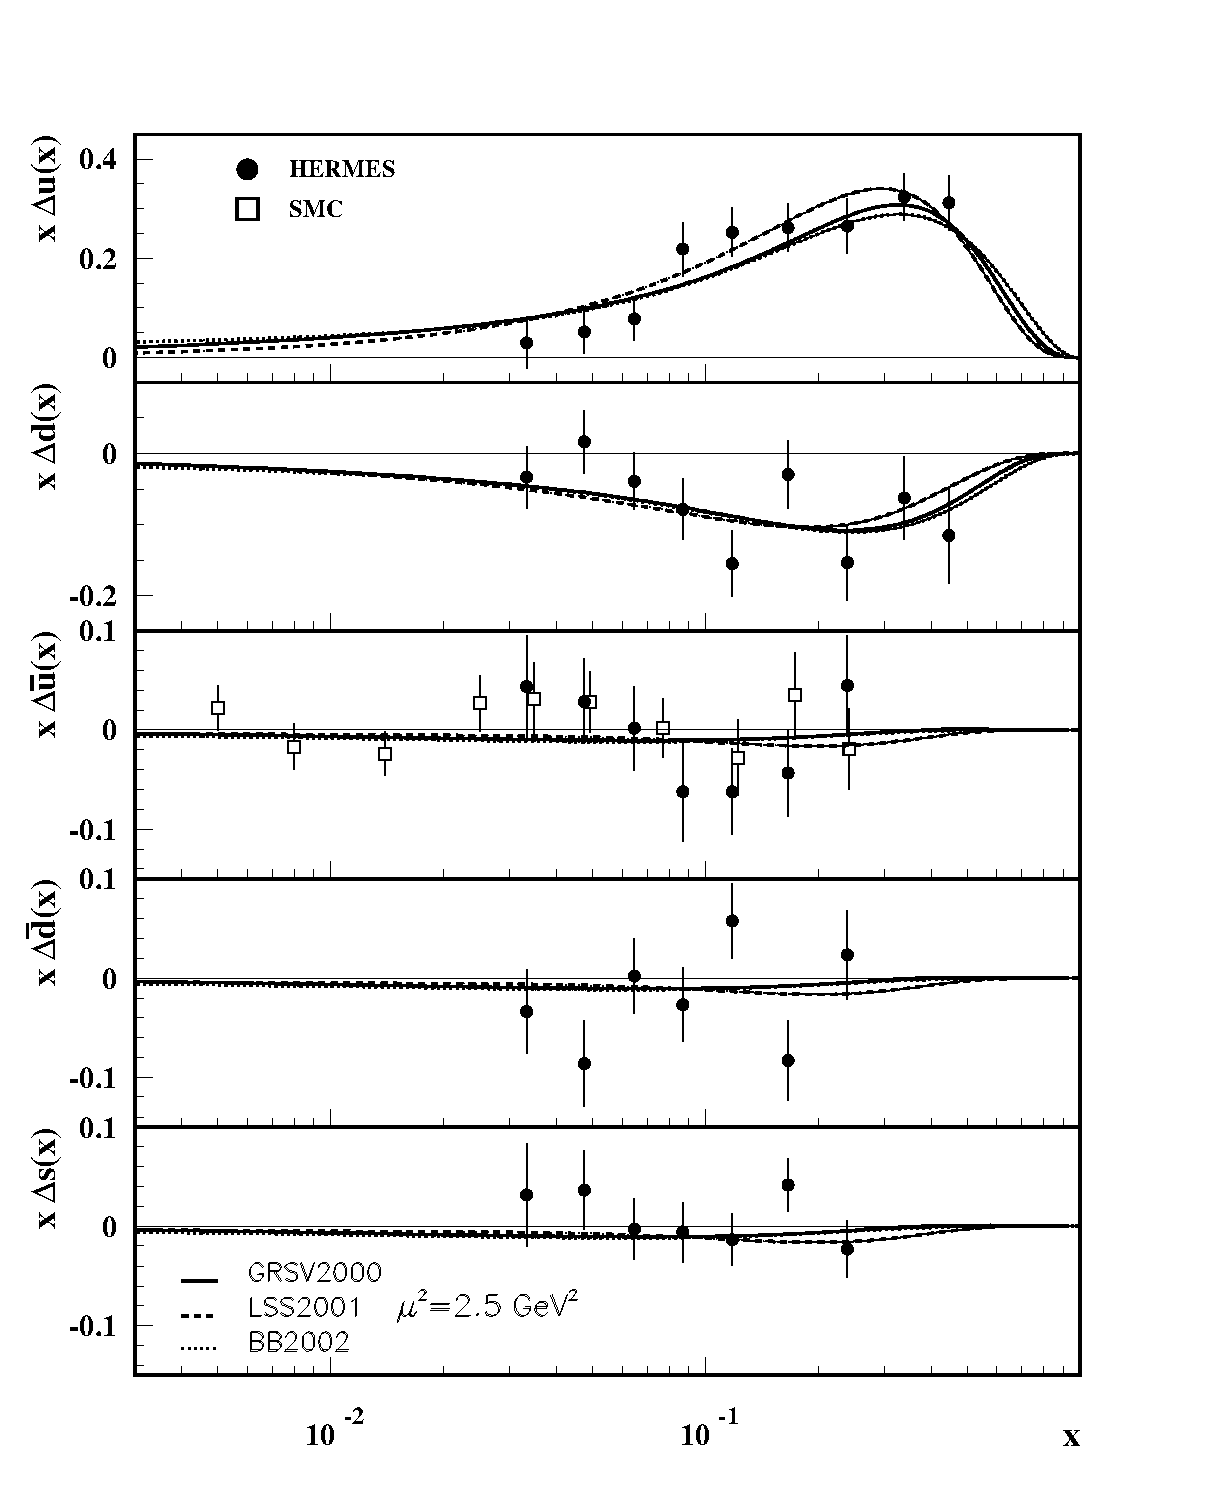
\includegraphics[width=1.0\textwidth]{figures/pol_pdf_5}
  \caption{from the Particle Data Group \cite{Amsler:2008zzb}.  Data points are SIDIS measurements using positron (HERMES) and muon (SMC).  SMC results extracted assuming $\Delta \bar u(x) = \Delta \bar d(x)$}
  \label{fig:pol_pdf_5}
\end{figure}

\begin{figure}
  \includegraphics[width=1.0\textwidth]{figures/aac03}
  \caption{\cite{Hirai:2003pm}  BB \cite{Bluemlein:2002be} uses ISET=3, LSS \cite{Leader:2001kh} uses $\bar{MS}$, GRSV \cite{Gluck:2000dy} uses STD.  But this is of course \textit{not} the most recent polarized PDF analysis using only DIS and SIDIS data.  My best guess at that is \cite{Leader:2006xc}}
\end{figure}

\begin{figure}
  \includegraphics[width=1.0\textwidth]{figures/lss06_deltag}
  \caption{Newest $\Delta g(x)$ using only DIS and SIDIS data that I'm aware of. \cite{Leader:2006xc}}
\end{figure}

Need to understand what constraints go into positive/negative/sign-changing $\Delta g(x)$ parameterizations.

\subsection{Photon-Gluon Fusion}

\begin{figure}
  \centering
  \begin{fmfgraph*}(200,150)
    \fmfleft{proton,gamma}
    \fmfright{proton',quark1,quark2}
    \fmf{fermion,width=2.5}{proton,v1}
    \fmf{fermion}{v1,proton'}
    \fmf{gluon}{v1,v2}
    \fmfblob{.15w}{v1}
    \fmf{fermion}{v2,quark1}
    \fmf{fermion}{v2,v3,quark2}
    \fmf{photon}{gamma,v3}

    % wow, it really feels like I should not have to do all of this
    \fmffixedx{0.}{v2,v3}
    \fmffixedy{0.}{v2,quark1}
    \fmffixedy{0.}{v3,quark2}
    \fmffixedy{0.}{v1,proton'}
    \fmffreeze
    \fmfshift{(0,-0.2h)}{v3}
    \fmfshift{(0.09w,-0.2h)}{quark2}
    \fmfshift{0,0.15h}{v1,proton'}
    
    % finally, add lines for outgoing quarks in struck proton
    \fmfi{plain}{vpath (__v1, __proton') shifted (thick*(-0.5,3.5))}
    \fmfi{plain}{vpath (__v1, __proton') shifted (thick*(-0.5,-3.5))}
  \end{fmfgraph*}
  \caption{Feynman diagram of photon-gluon fusion process}
\end{figure}


What's the problem with NLO analysis of these measurements?

Latest result from COMPASS analysis seems to be $\Delta g(x)/g(x) = -0.49~\pm~0.27(stat)~\pm~0.11(syst)$ at a scale $\mu^2 \sim 13 (GeV/c)^2$ and at an average gluon momentum fraction $<x>~\sim 0.11$ \cite{Alekseev:2009ey}.

%% Direct \Delta G figure without preliminary results
% \begin{figure}
%   \includegraphics[width=1.0\textwidth]{figures/compass_deltag}
%   \caption{\cite{Alekseev:2009ey}}
% \end{figure}

\begin{figure}
  \includegraphics[width=1.0\textwidth]{figures/compass_deltag_with_prelim}
  \caption{this figure comes from DIS2008, but I don't see anything in SPIRES or the arXiv on it yet.  Kurek was the author}
\end{figure}
\subsection{Polarized Proton Collisions}

``A cross section is written in factorized form as a convolution of parton distribution functions and fragmentation functions with a partonic subprocess cross section''

Assumptions:
\begin{itemize}
  \item Cross section can be written in factorized form
  \item Universality of parton distribution functions
  \item Universality of fragmentation functions
  \item partonic cross section calculable in perturbative QCD
\end{itemize}

First bullet point relies on the next 3, of course.

\begin{equation}
  A_{LL} = \frac{\sum_{f_1,f_2,f}~\Delta f_1 \otimes \Delta f_2 \otimes \sigma^{f_1 f_2 \rightarrow f X'} \hat a_{LL}^{f_1 f_2 \rightarrow f X'} \otimes D_f}{\sum_{f_1,f_2,f}~f_1 \otimes f_2 \otimes \sigma^{f_1 f_2 \rightarrow f X'} \otimes D_f} 
\end{equation}

\begin{equation}
  \hat a_{LL}^{f_1 f_2 \rightarrow f X'} = \frac{\Delta \sigma^{f_1 f_2 \rightarrow f X'}}{\sigma^{f_1 f_2 \rightarrow f X'}}
\end{equation}

\begin{figure}\begin{center}
  \includegraphics[width=0.5\textwidth]{figures/partonic_asymmetry}
  \caption{\cite{Bunce:2000uv}}
\end{center}\end{figure}

